% !TeX program = XeLaTeX
% !TeX encoding = UTF-8
% !TeX spellcheck = pt_PT
% !TeX root = main
\documentclass[10pt,a4paper,final]{report}
\usepackage[portuguese]{babel}
\usepackage[utf8x]{inputenc}
\usepackage[T1]{fontenc}
\usepackage{newtxtext,newtxmath} %TimesNewRoman
\usepackage[backend=biber,citestyle=numeric,sorting=none,style=ieee]{biblatex}
\usepackage[a4paper,top=3cm,bottom=2cm,left=3cm,right=3cm,marginparwidth=2cm]{geometry}
\usepackage{amsmath}
\usepackage{graphicx}
\usepackage[svgnames]{xcolor}
\usepackage{listings}
\usepackage[colorinlistoftodos]{todonotes}
\usepackage[colorlinks=true,allcolors=ipbbrown]{hyperref}
\usepackage{adjustbox}
\usepackage[pagestyles]{titlesec}
\usepackage[final]{pdfpages}
\usepackage{placeins}

\addbibresource{main.bib}

\titleformat{\chapter}[display]{\normalfont\bfseries}{}{0pt}{\Huge}
\newpagestyle{mystyle}
{\sethead[\thepage][][\chaptertitle]{}{}{\thepage}}
\pagestyle{mystyle}

% school colours
\definecolor{ipbgreen}{RGB}{166,204,59}
\definecolor{ipbbrown}{RGB}{153,80,42}
\definecolor{estigred}{RGB}{150,0,24}

\title{
  
\includegraphics[scale=0.5]{resources/ipbeja_logo.png}\\[0.5cm]
  Exemplo de Relatório
} % Doc name
\author{Gonçalo Amaro -- 17440\\João Saragoça -- 24123\\João Macedo -- 24572} % Doc's author/s
\date{16 de Novembro, 2022} % Doc date

\def\blankpage{%
      \clearpage%
      \thispagestyle{empty}%
      \addtocounter{page}{-1}%
      \null%
      \clearpage
}


\begin{document}

\maketitle

\blankpage{}

{
  \hypersetup{linkcolor=black}
  \tableofcontents
}

% \newpage
%
% {
%   \hypersetup{linkcolor=black}
%   \listoffigures
%   \listoftables
% }

\newpage

\chapter{Introdução}

\section{História}

\section{Princípios da encriptação quântica}

\textit{artigos: "Principios da Criptografia Quantica, Quantum Key Distribution Protocol, Ataques quanticos"}

\chapter{Limitações}

\section{Limitações conhecidas}

\textit{artigos: "On the Quantum Mechanical Bound on the Loss of Information through Side Channels in Quantum Cryptography", "Limitations on Practical Quantum Cryptography"}

\section{Propostas de mitigação das limitações}

\textit{artigo: "Quantum cryptography beyond quantum key distribution"}

\chapter{Protocolos usados na criptografia quântica}

Na criptografia quântica, os protocolos são as regras e procedimentos usados para codificar, transmitir e descodificar informações em um canal quântico. Esses protocolos são baseados nos princípios da mecânica quântica e são projetados para serem seguros contra uma variedade de ataques.

Um dos principais protocolos na criptografia quântica é o protocolo Quantum Key Distribution (QKD). Este protocolo permite a troca segura de chaves criptográficas em um canal quântico e é baseado nos princípios da mecânica quântica.

O protocolo QKD usa fotões para codificar e transmitir informações e é projetado para ser seguro contra uma variedade de ataques, incluindo aqueles que exploram as leis da física clássica. Além disso, os protocolos QKD também são projetados para serem resistentes a perdas e ruídos, permitindo uma comunicação segura em longas distâncias e em ambientes desafiadores.

Existem vários protocolos QKD diferentes que foram propostos e estudados, incluindo o protocolo BB84, o protocolo B92, o protocolo E91 e o protocolo SARG04. Cada um desses protocolos tem seus próprios recursos e vantagens exclusivos e pode ser mais adequado para diferentes aplicações e cenários.

Além dos protocolos QKD, também existem outros protocolos usados na criptografia quântica, como o protocolo OTP e o protocolo de autenticação baseado em BB84. Esses protocolos oferecem diferentes recursos e capacidades e podem ser úteis em aplicações ou cenários específicos.

\begin{figure}[!hbt]
  \centering
  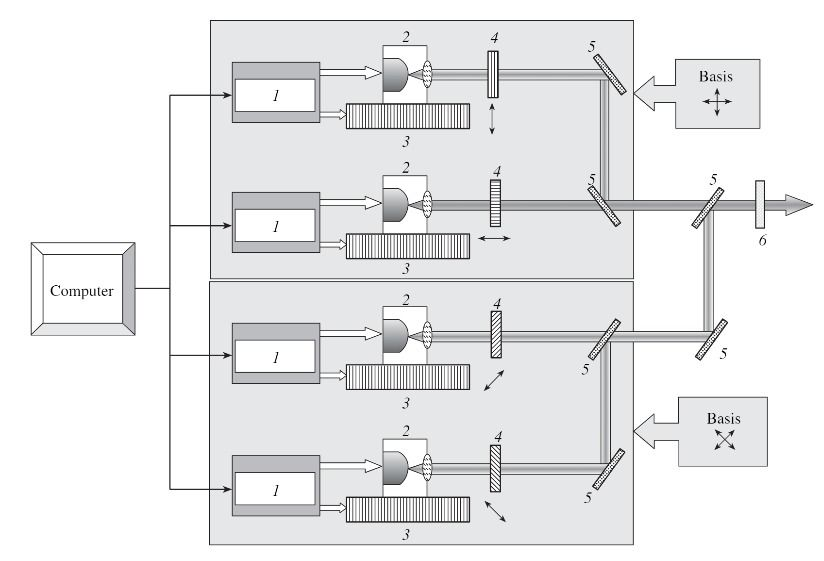
\includegraphics[width=\textwidth]{images/foton-pipeline.jpg}
  \caption{Figura informativa gráfica de uma arquitetura de canal quântico.}
  \label{fig:qkd-pipeline}
\end{figure}
\FloatBarrier

\section{Protocolos de Geração e Distribuição de Chaves}

O protocolo de geração e distribuição de chaves é uma parte fundamental de qualquer sistema criptográfico quântico. Este protocolo é responsável por criar e distribuir as chaves criptográficas que são usadas para codificar e descodificar as informações transmitidas por um canal quântico.

Um dos protocolos de geração e distribuição de chaves mais amplamente utilizados na criptografia quântica é o protocolo Quantum Key Distribution (QKD). Este protocolo permite a troca segura de chaves criptográficas em um canal quântico e é baseado nos princípios da mecânica quântica.

O protocolo QKD usa fotões para codificar e transmitir informações e é projetado para ser seguro contra uma variedade de ataques, incluindo aqueles que exploram as leis da física clássica. Além disso, os protocolos QKD também são projetados para serem resistentes a perdas e ruídos, permitindo uma comunicação segura em longas distâncias e em ambientes desafiadores.

Existem vários protocolos QKD diferentes que foram propostos e estudados, incluindo o protocolo BB84, o protocolo B92, o protocolo E91 e o protocolo SARG04. Cada um desses protocolos tem seus próprios recursos e vantagens exclusivos e pode ser mais adequado para diferentes aplicações e cenários.

Além dos protocolos QKD, também existem outros protocolos de geração e distribuição de chaves que foram propostos e estudados. Por exemplo, alguns pesquisadores exploraram o uso do protocolo OTP, que oferece segurança e desempenho aprimorados em comparação com os protocolos QKD tradicionais.

\subsection{Protocolo BB84}

O protocolo BB84, nomeado após seus inventores Charles Bennett e Gilles Brassard, é um conhecido protocolo de distribuição de chaves quânticas (QKD). Nesse protocolo, o remetente e o destinatário compartilham uma chave secreta trocando estados quânticos por um canal quântico. A chave é gerada medindo os estados usando um dos dois observáveis conjugados, escolhidos aleatoriamente.

A segurança do protocolo BB84 reside no fato de que qualquer tentativa de medir os estados quânticos irá perturbá-los, impossibilitando que um invasor obtenha a chave sem ser detectado. Isso é conhecido como o princípio da não-clonagem quântica.

O protocolo BB84 foi extensivamente estudado e demonstrou ser seguro contra vários tipos de ataques, incluindo ataques de intercepção e reenvio e ataques baseados em entrelaçamento. No entanto, como todos os protocolos QKD, é suscetível à perda de informações por meio de canais laterais, como perda de fotões no canal quântico. As propostas para mitigar essa limitação incluem o uso de códigos de correção de erros e estados de chamariz.

\begin{figure}[!hbt]
  \centering
  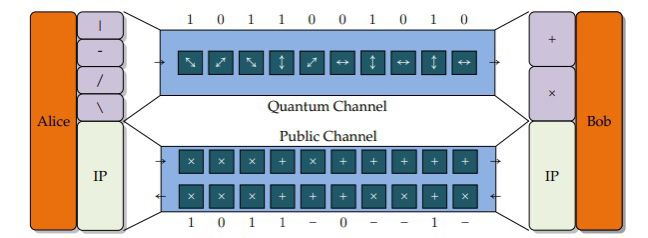
\includegraphics[width=\textwidth]{images/bb84.jpg}
  \caption{Figura ilustrativa do protocolo BB84. O remetente e o destinatário compartilham uma chave secreta trocando estados quânticos por um canal quântico. A chave é gerada medindo os estados usando um dos dois observáveis conjugados, escolhidos aleatoriamente.}
  \label{fig:bb84}
\end{figure}
\FloatBarrier

\subsection{Protocolo B92}

O protocolo B92 é outro protocolo conhecido de distribuição de chaves quânticas (QKD). Foi proposto por Charles Bennett em 1992 como uma versão simplificada do protocolo BB84.

No protocolo B92, o remetente e o destinatário compartilham uma chave secreta trocando estados quânticos por um canal quântico. A chave é gerada medindo os estados usando um dos dois observáveis conjugados, escolhidos aleatoriamente. No entanto, ao contrário do protocolo BB84, o remetente envia apenas um estado e o destinatário escolhe aleatoriamente com qual observável medi-lo.

A segurança do protocolo B92 baseia-se nos mesmos princípios do protocolo BB84: a impossibilidade de medir estados quânticos sem perturbá-los e o uso de observáveis conjugados para detectar qualquer distúrbio. No entanto, o protocolo B92 é mais simples e requer menos estados quânticos para serem trocados, tornando-o potencialmente mais prático para algumas aplicações.

Assim como o protocolo BB84, o protocolo B92 é suscetível à perda de informações por meio de canais laterais e outros ataques. Os pesquisadores estudaram várias maneiras de mitigar essas limitações, como o uso de estados de chamariz e códigos de correção de erros.

\subsection{Protocolo E91}

O protocolo E91, também conhecido como esquema E91, é um protocolo de distribuição de chave quântica (QKD) proposto por Artur Ekert em 1991. É uma variante do protocolo BB84 que usa estados quânticos baseados em entrelaçamento em vez de fotões individuais.

No protocolo E91, o remetente e o destinatário compartilham um par de partículas emaranhadas. O remetente mantém uma partícula e envia a outra para o receptor. Eles então usam suas partículas para gerar uma chave secreta, medindo-as usando um dos dois observáveis conjugados, escolhidos aleatoriamente.

A segurança do protocolo E91 baseia-se nos mesmos princípios do protocolo BB84: a impossibilidade de medir estados quânticos sem perturbá-los e o uso de observáveis conjugados para detectar qualquer distúrbio. No entanto, o protocolo E91 tem a vantagem de ser imune a certos tipos de ataques, como ataques de intercepção e reenvio, devido ao entrelaçamento das partículas.

Assim como os protocolos BB84 e B92, o protocolo E91 é suscetível à perda de informações por meio de canais laterais e outros ataques. Os pesquisadores estudaram várias maneiras de mitigar essas limitações, como o uso de estados de chamariz e códigos de correção de erros.

\begin{figure}[!hbt]
  \centering
  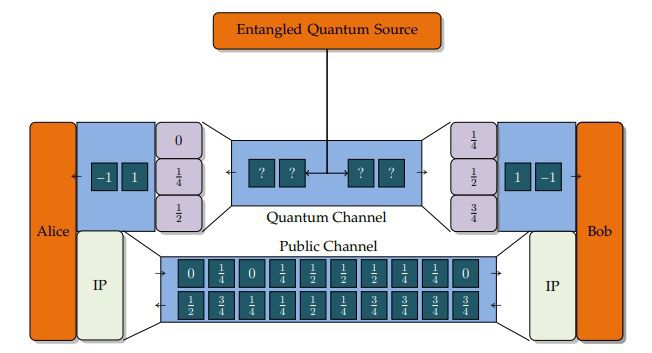
\includegraphics[width=\textwidth]{images/e91.jpg}
  \caption{Figura ilustrativa do protocolo E91. O remetente e o destinatário compartilham um par de partículas emaranhadas. O remetente mantém uma partícula e envia a outra para o receptor. Eles então usam suas partículas para gerar uma chave secreta, medindo-as usando um dos dois observáveis conjugados, escolhidos aleatoriamente.}
  \label{fig:e91}
\end{figure}
\FloatBarrier

\subsection{Protocolo SARG04}

O protocolo SARG04, também conhecido como protocolo de quatro estados, é um protocolo de distribuição de chave quântica (QKD) proposto por Stefano Pironio, Antonio Acin, Nicolas Gisin e Valerio Scarani em 2004. É uma variante do BB84 e B92 protocolos que usam quatro estados quânticos em vez de dois.

No protocolo SARG04, o remetente e o destinatário compartilham uma chave secreta trocando estados quânticos por um canal quântico. A chave é gerada medindo os estados usando um dos quatro observáveis conjugados, escolhidos aleatoriamente. Os quatro estados são escolhidos de forma que o remetente e o destinatário possam verificar a correção da chave por meio de um teste simples.

A segurança do protocolo SARG04 baseia-se nos mesmos princípios dos protocolos BB84 e B92: a impossibilidade de medir estados quânticos sem perturbá-los e o uso de observáveis conjugados para detectar qualquer distúrbio. O uso de quatro estados em vez de dois permite que o protocolo seja mais resistente a certos tipos de ataques, como o ataque de intercepção e reenvio.

Como os outros protocolos QKD, o protocolo SARG04 é suscetível à perda de informações por meio de canais laterais e outros ataques. Os pesquisadores estudaram várias maneiras de mitigar essas limitações, como o uso de estados de chamariz e códigos de correção de erros.

\begin{figure}[!hbt]
  \centering
  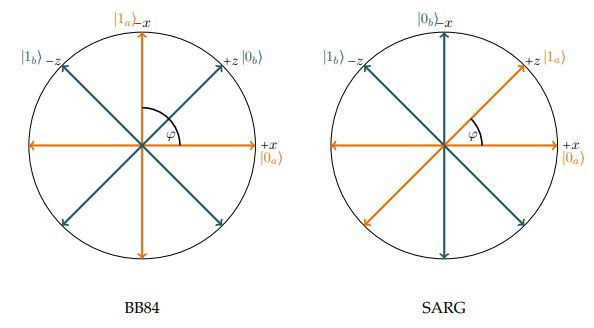
\includegraphics[width=\textwidth]{images/bb84-vs-sarg04.jpg}
  \caption{Figura comparativa entre os protocolos BB84 e SARG04 no que diz respeito à segurança. O protocolo BB84 é mais suscetível a ataques de intercepção e reenvio, enquanto o protocolo SARG04 é mais suscetível a ataques de canal lateral.}
  \label{fig:bb84-vs-sarg04}
\end{figure}
\FloatBarrier

\subsection{Protocolo OTP}

O protocolo OTP, ou protocolo one-time pad (OTP), é um protocolo de criptografia clássico que fornece segurança incondicional. É um método simples e eficiente de encriptar mensagens usando uma chave secreta compartilhada.

No protocolo OTP, o remetente e o destinatário compartilham uma chave secreta tão longa quanto a mensagem que desejam encriptar. O remetente usa a chave para encriptar a mensagem executando uma operação OR (XOR) exclusiva entre a mensagem e a chave. O receptor pode então desencriptar a mensagem executando a mesma operação XOR usando a mesma chave.

A segurança do protocolo OTP depende do fato de que a chave é completamente aleatória e é usada apenas uma vez. Desde que a chave seja mantida em segredo e seja usada apenas para uma única mensagem, o protocolo é teoricamente inquebrável, mesmo por um invasor com poder computacional ilimitado.

No contexto dos protocolos de distribuição de chaves quânticas (QKD), o protocolo OTP pode ser usado para aprimorar a segurança e o desempenho dos sistemas QKD. Por exemplo, o protocolo OTP pode ser usado para encriptar a chave secreta gerada por um protocolo QKD, fornecendo uma camada adicional de segurança.

O protocolo OTP tem várias vantagens sobre os protocolos QKD tradicionais. É simples e eficiente e oferece segurança incondicional, desde que a chave seja mantida em segredo e usada apenas uma vez. Além disso, não possui as mesmas limitações dos protocolos QKD, como a suscetibilidade à perda de informações por canais laterais.

No entanto, o protocolo OTP também possui várias limitações práticas que devem ser consideradas ao usá-lo em combinação com protocolos QKD. A chave deve ser compartilhada com segurança entre o remetente e o destinatário e deve ser mantida em segredo de todas as outras partes. A chave também deve ser tão longa quanto a mensagem, o que pode ser impraticável para mensagens longas. Além disso, a chave deve ser usada apenas uma vez, portanto, uma nova chave deve ser gerada para cada mensagem.

\section{Protocolos de Autenticação}

No campo da criptografia quântica, os protocolos de autenticação são métodos de verificação segura da identidade de um usuário ou dispositivo em uma rede usando os princípios da mecânica quântica. Eles são uma parte importante dos sistemas de distribuição de chaves quânticas (QKD), pois ajudam a impedir o acesso não autorizado e protegem contra vários tipos de ataques, como personificação e ataques man-in-the-middle.

Existem vários protocolos de autenticação diferentes que foram propostos e estudados para uso em criptografia quântica, cada um com seus pontos fortes e fracos. Alguns protocolos de autenticação comuns para criptografia quântica incluem:

\begin{itemize}
  \item Autenticação quântica, na qual um usuário comprova sua identidade trocando estados quânticos com o verificador
  \item Protocolos de acordo de chave quântica, nos quais duas partes estabelecem uma chave secreta compartilhada trocando estados quânticos
  \item Assinaturas digitais quânticas, nas quais um usuário comprova sua identidade assinando uma mensagem com um estado quântico
  \item Infraestrutura quântica de chave pública (PKI), na qual usuários e dispositivos recebem certificados digitais que são verificados usando estados quânticos
\end{itemize}

Esses protocolos de autenticação podem fornecer segurança aprimorada em comparação aos protocolos de autenticação clássicos, pois são baseados nos princípios da mecânica quântica e, portanto, imunes a certos tipos de ataques. No entanto, eles também têm suas próprias limitações e desafios, como a necessidade de hardware quântico especializado e a suscetibilidade à perda de informações por canais secundários.

\subsection{Autenticação Quântica}

A autenticação quântica é um método de verificação segura da identidade de um usuário ou dispositivo em um sistema de distribuição de chave quântica (QKD) usando os princípios da mecânica quântica. Na autenticação quântica, o usuário e o verificador trocam estados quânticos, e o usuário prova sua identidade medindo e respondendo corretamente aos estados.

A autenticação quântica tem várias vantagens sobre os métodos de autenticação clássicos, como autenticação baseada em senha ou autenticação biométrica. Por ser baseado nos princípios da mecânica quântica, é imune a certos tipos de ataques, como ataques de dicionário e ataques man-in-the-middle. Além disso, não exige que o usuário se lembre de uma senha ou possua um token físico, tornando-o potencialmente mais conveniente e fácil de usar.

No entanto, a autenticação quântica também tem seus próprios desafios e limitações. Requer que o usuário e o verificador tenham acesso a hardware quântico especializado, como detectores de fotão único ou fontes de entrelaçamento. Além disso, é suscetível à perda de informações por meio de canais laterais, como perda de fotões no canal quântico.

\subsection{Protocolos de Acordo de Chave Quântica}

Os protocolos de acordo de chave quântica são métodos de estabelecer com segurança uma chave secreta compartilhada entre duas partes usando os princípios da mecânica quântica. Num protocolo de acordo de chave quântica, as duas partes trocam estados quânticos e a chave é gerada realizando medições nos estados.

Os protocolos de acordo de chave quântica têm várias vantagens sobre os protocolos clássicos de acordo de chave, como a troca de chaves Diffie-Hellman. Por serem baseados nos princípios da mecânica quântica, eles são imunes a certos tipos de ataques, como ataques man-in-the-middle e ataques de personificação. Além disso, eles não exigem que as partes tenham um segredo compartilhado anteriormente, tornando-os potencialmente mais práticos e amigáveis.

No entanto, os protocolos de acordo de chave quântica também têm seus próprios desafios e limitações. Eles exigem que as partes tenham acesso a hardware quântico especializado, como detectores de fotão único ou fontes de entrelaçamento. Além disso, eles são suscetíveis à perda de informações por meio de canais laterais, como perda de fotões no canal quântico.

\subsubsection{Troca de chaves Diffie-Hellman}

A troca de chaves Diffie-Hellman (troca de chaves D-H) é um protocolo de criptografia clássico que permite que duas partes estabeleçam uma chave secreta compartilhada em um canal inseguro. Foi proposto pela primeira vez por Whitfield Diffie e Martin Hellman em 1976 e é amplamente utilizado em muitos sistemas criptográficos.

Na troca de chaves D-H, as duas partes, Alice e Bob, concordam com um grande número primo, p, e uma raiz primitiva, g, de p. Alice então escolhe um inteiro secreto, a, e calcula \(g^a \mod p\). Bob escolhe um inteiro secreto, b, e calcula \(g^b \mod p\). Alice e Bob então trocam \(g^a \mod p e g^b \mod p\), respectivamente.

Depois de trocar esses valores, Alice calcula \(g^b \mod p\) e Bob calcula \(g^a \mod p\). Devido às propriedades da aritmética modular, esses dois valores são iguais e formam a chave secreta compartilhada.

A troca de chaves D-H apresenta diversas vantagens, como sua simplicidade e eficiência. Não exige que as partes tenham um segredo compartilhado anteriormente e fornece confidencialidade, pois a chave secreta compartilhada nunca é transmitida pelo canal.

Embora os protocolos de troca de chaves D-H e acordo de chaves quânticas sirvam ao mesmo propósito geral de estabelecer uma chave secreta compartilhada, eles diferem nas suas propriedades e limitações de segurança. A troca de chaves D-H é vulnerável a certos tipos de ataques, como ataques man-in-the-middle, enquanto os protocolos de acordo de chaves quânticas são imunes a esses ataques. Além disso, a troca de chaves D-H não é resistente à perda de informações por meio de canais laterais, enquanto os protocolos de acordo de chave quântica podem ser resistentes a esse tipo de ataque, dependendo do protocolo e implementação específicos.

\subsection{Assinaturas Digitais Quânticas}

As assinaturas digitais quânticas são um método de assinatura segura de mensagens digitais usando os princípios da mecânica quântica. Num esquema de assinatura digital quântica, o usuário prova sua identidade assinando a mensagem com um estado quântico, e o verificador verifica a assinatura medindo o estado.

As assinaturas digitais quânticas têm várias vantagens sobre as assinaturas digitais clássicas, como as assinaturas RSA. Por serem baseados nos princípios da mecânica quântica, eles são imunes a certos tipos de ataques, como ataques de falsificação e ataques de representação. Além disso, eles não exigem que o usuário possua uma chave privada, tornando-os potencialmente mais convenientes e fáceis de usar.

No entanto, as assinaturas digitais quânticas também têm seus próprios desafios e limitações. Eles exigem que o usuário e o verificador tenham acesso a hardware quântico especializado, como detectores de fotão único ou fontes de entrelaçamento. Além disso, eles são suscetíveis à perda de informações por meio de canais laterais, como perda de fotões no canal quântico.

\subsection{Infraestrutura de Chave Públicas Quânticas}

A infraestrutura de chave pública quântica (PKI) é um método de emissão, gestão e verificação segura de certificados digitais usando os princípios da mecânica quântica. Num sistema PKI quântico, os usuários e dispositivos recebem certificados digitais que são verificados usando estados quânticos.

O Quantum PKI tem várias vantagens sobre os sistemas clássicos de PKI, como o uso de RSA ou criptografia de curva elíptica. Por ser baseado nos princípios da mecânica quântica, é imune a certos tipos de ataques, como ataques de falsificação e ataques de representação. Além disso, não exige que o usuário ou o verificador possua uma chave privada, tornando-o potencialmente mais conveniente e amigável.

No entanto, a PKI quântica também tem seus próprios desafios e limitações. Requer que o usuário, o verificador e a autoridade certificadora tenham acesso a hardware quântico especializado, como detectores de fotão único ou fontes de entrelaçamento. Além disso, é suscetível à perda de informações por meio de canais laterais, como perda de fotões no canal quântico.

\newpage

\chapter{Ataques}

A criptografia quântica é um campo que se encontra ainda em desenvolvimento e, como tal, está sujeito a vários tipos de ataques que podem comprometer a segurança dos sistemas de distribuição de chaves quânticas (QKD). Esses ataques podem ser amplamente classificados em duas categorias: ataques no canal quântico e ataques no canal clássico.

\section{Tipos de Ataques}

\subsection{Ataques no Canal Quântico}

Os ataques ao canal quântico visam a transmissão de estados quânticos pelo canal e podem assumir várias formas. Por exemplo, um invasor pode tentar interceptar e medir os estados quânticos para obter informações sobre a chave secreta. Isso é conhecido como ataque de intercepção e medição, e é um tipo de ataque man-in-the-middle.

Outro tipo de ataque no canal quântico é um ataque de divisão do número de fotões, no qual o atacante divide os fotões no estado quântico e mede cada metade separadamente. Isso permite que o invasor obtenha informações parciais sobre a chave secreta sem ser detectado pelas partes legítimas.

\subsection{Ataques no Canal Clássico}

Os ataques no canal clássico visam a transmissão de informações clássicas pelo canal, como mensagens de autenticação ou informações de correção de erros. Esses ataques podem assumir várias formas, como ataques de personificação, nos quais o invasor finge ser uma das partes legítimas para obter acesso à chave secreta.

Outro tipo de ataque ao canal clássico é o ataque man-in-the-middle, no qual o invasor intercepta a informação clássica e a modifica para obter acesso à chave secreta. Esse tipo de ataque pode ser difícil de detectar, pois o invasor pode manipular as informações clássicas de forma que pareçam válidas para as partes legítimas.

\begin{figure}[!hbt]
  \centering
  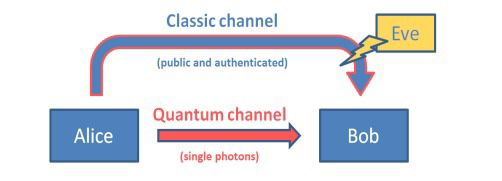
\includegraphics[width=\textwidth]{images/possible-attack.jpg}
  \caption{Figura ilustrativa de um ataque ao canal clássico.}
  \label{fig:classic-attack}
\end{figure}
\FloatBarrier

\section{Ataques Conhecidos}

Existem vários métodos conhecidos de ataque em criptografia quântica, que visam vários aspectos dos sistemas QKD. Esses métodos incluem:

\begin{itemize}
  \item Ataques de intercepção e medição, nos quais o invasor intercepta e mede os estados quânticos para obter informações sobre a chave secreta.
  \item Ataques de divisão do número de fotões, nos quais o atacante divide os fotões no estado quântico e mede cada metade separadamente.
  \item Ataques de personificação, nos quais o invasor finge ser uma das partes legítimas para obter acesso à chave secreta.
  \item Ataques man-in-the-middle, em que o invasor intercepta e modifica informações clássicas para obter acesso à chave secreta.
  \item Ataques de canal lateral, nos quais o invasor usa informações obtidas por meio de canais laterais, como perda de fotões no canal quântico, para obter informações sobre a chave secreta.
\end{itemize}

\subsection{Ataques de Intercepção e Medição}

Um ataque de intercepção e medição é um tipo de ataque em criptografia quântica que visa a transmissão de estados quânticos pelo canal. Num ataque de intercepção e medição, o invasor intercepta os estados quânticos e os mede para obter informações sobre a chave secreta.

Esse tipo de ataque é uma forma de ataque man-in-the-middle, pois o invasor é capaz de manipular a comunicação entre as partes legítimas sem ser detectado. Como o invasor está medindo os estados quânticos, ele pode obter informações parciais sobre a chave secreta sem ser detectado pelas partes legítimas.

Existem vários métodos conhecidos de detecção e mitigação de ataques de intercepção e medição. Por exemplo, códigos de correção de erros quânticos podem ser usados para detectar e corrigir erros nos estados quânticos, como perda de fotões ou erros de fase. Além disso, a autenticação quântica pode ser usada para verificar a identidade das partes envolvidas no sistema QKD e evitar ataques de representação.

\subsection{Ataques de Divisão do Número de Fotões}

Um ataque de divisão de número de fotões é um tipo de ataque em criptografia quântica que visa a transmissão de estados quânticos pelo canal. Num ataque de divisão do número de fotões, o atacante divide os fotões no estado quântico e mede cada metade separadamente. Isso permite que o invasor obtenha informações parciais sobre a chave secreta sem ser detectado pelas partes legítimas.

Os ataques de divisão do número de fotões são uma preocupação particular em sistemas QKD que usam estados coerentes fracos, pois esses estados são compostos de uma superposição de diferentes números de fotões. O atacante pode dividir o estado em duas partes, cada uma contendo um número diferente de fotões, e medir cada parte separadamente. Isso permite que o invasor obtenha informações parciais sobre a chave secreta, sem ser detectado pelas partes legítimas.

Existem vários métodos conhecidos de detecção e mitigação de ataques de divisão do número de fotões. Por exemplo, códigos de correção de erros quânticos podem ser usados para detectar e corrigir erros nos estados quânticos, como perda de fotões ou erros de fase. Além disso, a autenticação quântica pode ser usada para verificar a identidade das partes envolvidas no sistema QKD e evitar ataques de representação.

\begin{figure}[!hbt]
  \centering
  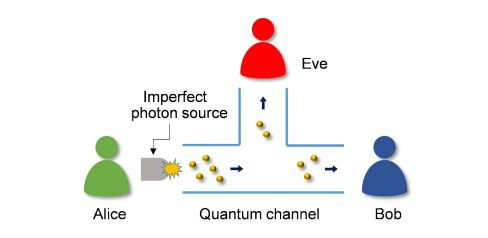
\includegraphics[width=\textwidth]{images/foton-division-attack.jpg}
  \caption{Figura ilustrativa de um ataque de divisão do número de fotões. O atacante divide o estado quântico em duas partes, cada uma contendo um número diferente de fotões. O atacante mede cada parte separadamente para obter informações parciais sobre a chave secreta.}
  \label{fig:foton-division-attack}
\end{figure}
\FloatBarrier

\subsection{Ataques de Personificação}

Um ataque de personificação é um tipo de ataque em criptografia quântica que tem como alvo as informações clássicas transmitidas pelo canal. Num ataque de personificação, o invasor finge ser uma das partes legítimas para obter acesso à chave secreta.

Esse tipo de ataque pode ser difícil de detectar, pois o invasor pode manipular as informações clássicas de forma que pareçam válidas para as partes legítimas. Por exemplo, o invasor pode usar uma identidade falsa para se autenticar para a outra parte ou pode modificar as mensagens de autenticação para obter acesso à chave secreta.

Existem vários métodos conhecidos de detecção e mitigação de ataques de personificação. Por exemplo, a autenticação quântica pode ser usada para verificar a identidade das partes envolvidas no sistema QKD e evitar ataques de personificação. Além disso, protocolos criptográficos, como protocolos de autenticação ou protocolos de troca de chaves, podem ser usados para fornecer segurança adicional e proteção contra ataques no canal clássico.

\subsection{Ataques de Canal Lateral}

Um ataque de canal lateral é um tipo de ataque em criptografia quântica que usa informações obtidas por meio de canais laterais, como perda de fotões no canal quântico, para obter informações sobre a chave secreta.

Os ataques de canal lateral podem ser difíceis de detectar, pois o invasor não manipula diretamente os estados quânticos ou as informações clássicas transmitidas pelo canal. Em vez disso, o invasor usa as informações obtidas por meio do canal lateral, como o tempo ou a intensidade dos fotões, para obter informações parciais sobre a chave secreta.

Existem vários métodos conhecidos de detecção e mitigação de ataques de canal lateral. Por exemplo, códigos de correção de erros quânticos podem ser usados para detectar e corrigir erros nos estados quânticos, como perda de fotões ou erros de fase. Além disso, os códigos clássicos de correção de erros podem ser usados para detectar e corrigir erros nas informações clássicas transmitidas pelo canal, como mensagens de autenticação ou informações de correção de erros.

\newpage

\section{Métodos de defesa e mitigação conhecidos}

Embora os ataques na criptografia quântica sejam uma ameaça significativa à segurança dos sistemas QKD, também existem vários métodos conhecidos de defesa e mitigação que podem ser usados para proteger contra esses ataques. Esses métodos incluem:

\begin{itemize}
  \item Códigos de correção de erros quânticos, que podem ser usados para detectar e corrigir erros nos estados quânticos, como perda de fotões ou erros de fase.
  \item Autenticação quântica, que pode ser usada para verificar a identidade das partes envolvidas no sistema QKD e evitar ataques de personificação.
  \item Protocolos de acordo de chave quântica, que podem ser usados para estabelecer uma chave secreta compartilhada entre as partes de forma segura e autenticada.
  \item Códigos de correção de erros clássicos, que podem ser usados para detectar e corrigir erros nas informações clássicas transmitidas pelo canal, como mensagens de autenticação ou informações de correção de erros.
  \item Protocolos criptográficos, como protocolos de autenticação ou protocolos de troca de chaves, que podem ser usados para fornecer segurança adicional e proteção contra ataques no canal clássico.
\end{itemize}

\subsection{Códigos de correção de erros quânticos}

Os códigos de correção de erros quânticos são um componente chave de muitos sistemas QKD e desempenham um papel crítico na detecção e correção de erros nos estados quânticos transmitidos.

Os códigos de correção de erros quânticos são baseados nos princípios da mecânica quântica e usam estados quânticos emaranhados para codificar e transmitir as informações. Isso permite que os estados quânticos sejam protegidos contra erros, como perda de fotões ou erros de fase, que podem ocorrer durante a transmissão.

Existem vários tipos diferentes de códigos de correção de erros quânticos, que usam diferentes esquemas de codificação e oferecem diferentes níveis de proteção contra erros. Por exemplo, alguns códigos são projetados para proteger contra a perda de um único fotão, enquanto outros são projetados para proteger contra a perda de múltiplos fotões.

\subsection{Autenticação quântica}

A autenticação quântica é uma técnica utilizada em sistemas QKD para verificar a identidade das partes envolvidas na comunicação.

A autenticação quântica é baseada nos princípios da mecânica quântica e usa estados quânticos emaranhados para codificar e transmitir as informações de autenticação. Isso permite que as informações de autenticação sejam protegidas contra ataques, como ataques de personificação ou man-in-the-middle, que podem tentar obter acesso à chave secreta.

Existem vários métodos diferentes de autenticação quântica, que usam diferentes esquemas de codificação e oferecem diferentes níveis de proteção contra ataques. Por exemplo, alguns métodos usam protocolos de acordo de chave quântica para estabelecer uma chave secreta compartilhada de maneira segura e autenticada, enquanto outros usam primitivas criptográficas quânticas, como assinaturas quânticas ou compromissos quânticos, para fornecer segurança adicional.

\subsection{Protocolos de acordo de chave quântica}

Os protocolos de acordo de chave quântica são uma classe de protocolos criptográficos projetados para estabelecer uma chave secreta compartilhada entre duas ou mais partes de maneira segura e autenticada.

Esses protocolos são baseados nos princípios da mecânica quântica e usam estados quânticos emaranhados para codificar e transmitir as informações de acordo de chave. Isso permite que as informações do acordo de chave sejam protegidas contra ataques, como ataques man-in-the-middle, que podem tentar obter acesso à chave secreta.

Existem vários protocolos diferentes de acordo de chave quântica, que usam diferentes esquemas de codificação e oferecem diferentes níveis de segurança e desempenho. Por exemplo, alguns protocolos são baseados nos princípios de distribuição de chave quântica (QKD), enquanto outros são baseados nos princípios de acordo de chave quântica (QKA).

\subsection{Códigos de correção de erros clássicos}

Os códigos clássicos de correção de erros são um componente chave de muitos sistemas QKD e desempenham um papel crítico na detecção e correção de erros nas informações clássicas transmitidas.

Os códigos clássicos de correção de erros são baseados nos princípios da teoria clássica da informação e usam algoritmos matemáticos para codificar e transmitir as informações. Isso permite que as informações sejam protegidas contra erros, como erros de transmissão ou interferência, que podem ocorrer durante a transmissão.

Existem vários tipos diferentes de códigos clássicos de correção de erros, que usam diferentes esquemas de codificação e oferecem diferentes níveis de proteção contra erros. Por exemplo, alguns códigos são projetados para proteger contra erros de bit único, enquanto outros são projetados para proteger contra erros de vários bits.

\subsection{Protocolos criptográficos}

Os protocolos criptográficos são uma classe de algoritmos usados para fornecer segurança e proteção em sistemas de comunicação. Esses protocolos são baseados nos princípios da criptografia e usam técnicas matemáticas, como criptografia e autenticação, para proteger as informações transmitidas pelo canal.

Os protocolos criptográficos são um componente importante de muitos sistemas QKD e fornecem segurança e proteção adicionais contra ataques no canal clássico. Por exemplo, os protocolos de autenticação podem ser usados para verificar a identidade das partes envolvidas na comunicação e para evitar a representação ou ataques man-in-the-middle. Além disso, os protocolos de troca de chaves podem ser usados para estabelecer uma chave secreta compartilhada de maneira segura e autenticada.

Existem vários protocolos criptográficos diferentes habitualmente usados em sistemas QKD, incluindo protocolos de autenticação, protocolos de troca de chaves e primitivas criptográficas, como assinaturas ou compromissos.

\newpage

\chapter{Prespectivas futuras}

\chapter{Conclusão}

Neste artigo, exploramos o campo da criptografia quântica, uma área em rápido desenvolvimento que usa os princípios da mecânica quântica para transmitir e proteger informações. Discutimos a história da criptografia quântica, os princípios subjacentes a esse campo e os principais protocolos usados na criptografia quântica.

Também discutimos as limitações e soluções potenciais para essas limitações e destacamos os muitos desafios e oportunidades que existem neste campo emocionante. Por fim, abordamos as perspectivas futuras da criptografia quântica e discutimos os muitos desenvolvimentos empolgantes que provavelmente ocorrerão nos próximos anos.

Concluindo, a criptografia quântica é um campo fascinante e em rápido desenvolvimento que tem o potencial de revolucionar a maneira como pensamos sobre a segurança da comunicação. Apesar dos muitos desafios que permanecem, a promessa da criptografia quântica é clara e é provável que esse campo continue a desempenhar um papel importante no futuro da comunicação segura.

\chapter{Webgrafia}

\printbibliography


\end{document}
